\documentclass[a4paper, 12pt]{article}
\usepackage[utf8]{inputenc}
\usepackage{graphicx}
\usepackage{subcaption}
\usepackage{float}
\usepackage{amsmath}
\usepackage{amssymb}
\usepackage{lipsum}
\usepackage{hyperref}
\setlength{\belowcaptionskip}{-10pt}
\DeclareMathSizes{10}{12}{12}{12}
\usepackage[margin=0.8in]{geometry}
\usepackage{color} %red, green, blue, yellow, cyan, magenta, black, white
\definecolor{mygreen}{RGB}{28,172,0} % color values Red, Green, Blue
\definecolor{mylilas}{RGB}{170,55,241}
\usepackage{listings}
\lstset{escapeinside={<@}{@>}}
\usepackage{cite}
\usepackage{url}
\usepackage{tikz}
\usepackage{booktabs}
\usetikzlibrary{automata, positioning}
\usepackage{fancyheadings}
\usepackage{dsfont}
\usepackage{mathrsfs}
\usepackage{afterpage}
\usepackage{physics}

\newenvironment{changemargin}[2]{%
\begin{list}{}{%
\setlength{\topsep}{0pt}%
\setlength{\leftmargin}{#1}%
\setlength{\rightmargin}{#2}%
\setlength{\listparindent}{\parindent}%
\setlength{\itemindent}{\parindent}%
\setlength{\parsep}{\parskip}%
}%
\item[]}{\end{list}}
%useful tool for hiding stuff that breaks
\iffalse %(starts environment)
%(hidden stuff)
\fi % (ends environment)

\lstset{language=R,%
    basicstyle=\ttfamily,
	frame=none,
    framesep=19pt,
    breaklines=true,%
    belowskip=0.5cm,
    aboveskip=0.5cm,
    morekeywords={matlab2tikz},
    keywordstyle=\color{blue},%
    morekeywords=[2]{1}, keywordstyle=[2]{\color{black}},
    identifierstyle=\color{black},%
    stringstyle=\color{mylilas},
    commentstyle=\color{mygreen},%
    showstringspaces=false,%without this there will be a symbol in the places where there is a space
    numbers=none,
    numberstyle={\tiny \color{black}},% size of the numbers
    numbersep=9pt, % this defines how far the numbers are from the text
    emph=[1]{for,end,break},emphstyle=[1]\color{red}, %some words to emphasise
    %emph=[2]{word1,word2}, emphstyle=[2]{style},    
}


\begin{document}
\section*{Intro}

We wish to identify cells with mitochondrial dysfunction by the expression of proteins present. \\
We have frozen tissues from patients with mitochondrial disease and tissues from `healthy' subjects. Our goal is to use a two component Gaussian mixture model (GMM) to classify patient fibres as `like control' and `not like control' and using a Bayesian approach for parameter inference. This allows us to calculate the proportion of deficient fibres. \\

We use information about from the control data to inform priors for the patient data. The posterior distributions for this is then used as a basis for the `like control' component of the GMM. 

\section*{The Model}
Let $\boldsymbol{Y}=\left( \log\text{VDAC1},\text{  } \log\text{[protein expression]}  \right)^T$ and 
\begin{equation}
    \boldsymbol{Y}_i = \pi \text{N}\left( \boldsymbol{\mu}_1, T_1 \right) + (1-\pi)\text{N}(\boldsymbol{\mu}_2, T_2).
\end{equation}
Let $Z_i$ be an auxiliary variable to note the component membership for observation $i$. We model this using a Bernoulli distribution with parameter $p$, such that
\begin{equation}
    Z_i \sim \text{Bern}(p).
\end{equation}

When modelling the control data, we fit the same two-component GMM but set $p=0$. This allows all fibres in the control to classified as `like control'. When modelling patient data we give $p$ a prior distribution, such that
\begin{equation}
    p = \begin{cases}
        \tilde{p}, & \text{if patient} \\
        0, & \text{if control}
    \end{cases}
\end{equation}
where $\tilde{p}\sim \text{Beta}(\alpha, \beta)$. The model parameters $\boldsymbol{\mu}_i$ and $T_i$ are given suitable bivariate normal distribution and Wishart distributions respectively.

\section*{Control Data}
\subsection*{Prior Beliefs}
The prior beliefs for the second component are arbitrary as setting $p=0$ means that inference can only be performed on the `like control' component, component one. Similarly prior beliefs for $\tilde{p}$ are also ignored here. 
\begin{center}
\begin{tabular}{c  c}
    $\boldsymbol{\mu}_1 \sim \text{N}\left(\begin{pmatrix}4\\4\end{pmatrix}, 4*I_2 \right)$ &  $T_1 \sim \text{Wishart}(2, 2*I_2)$ \\
\end{tabular}
\end{center}

\begin{figure}[H]
    \centering
    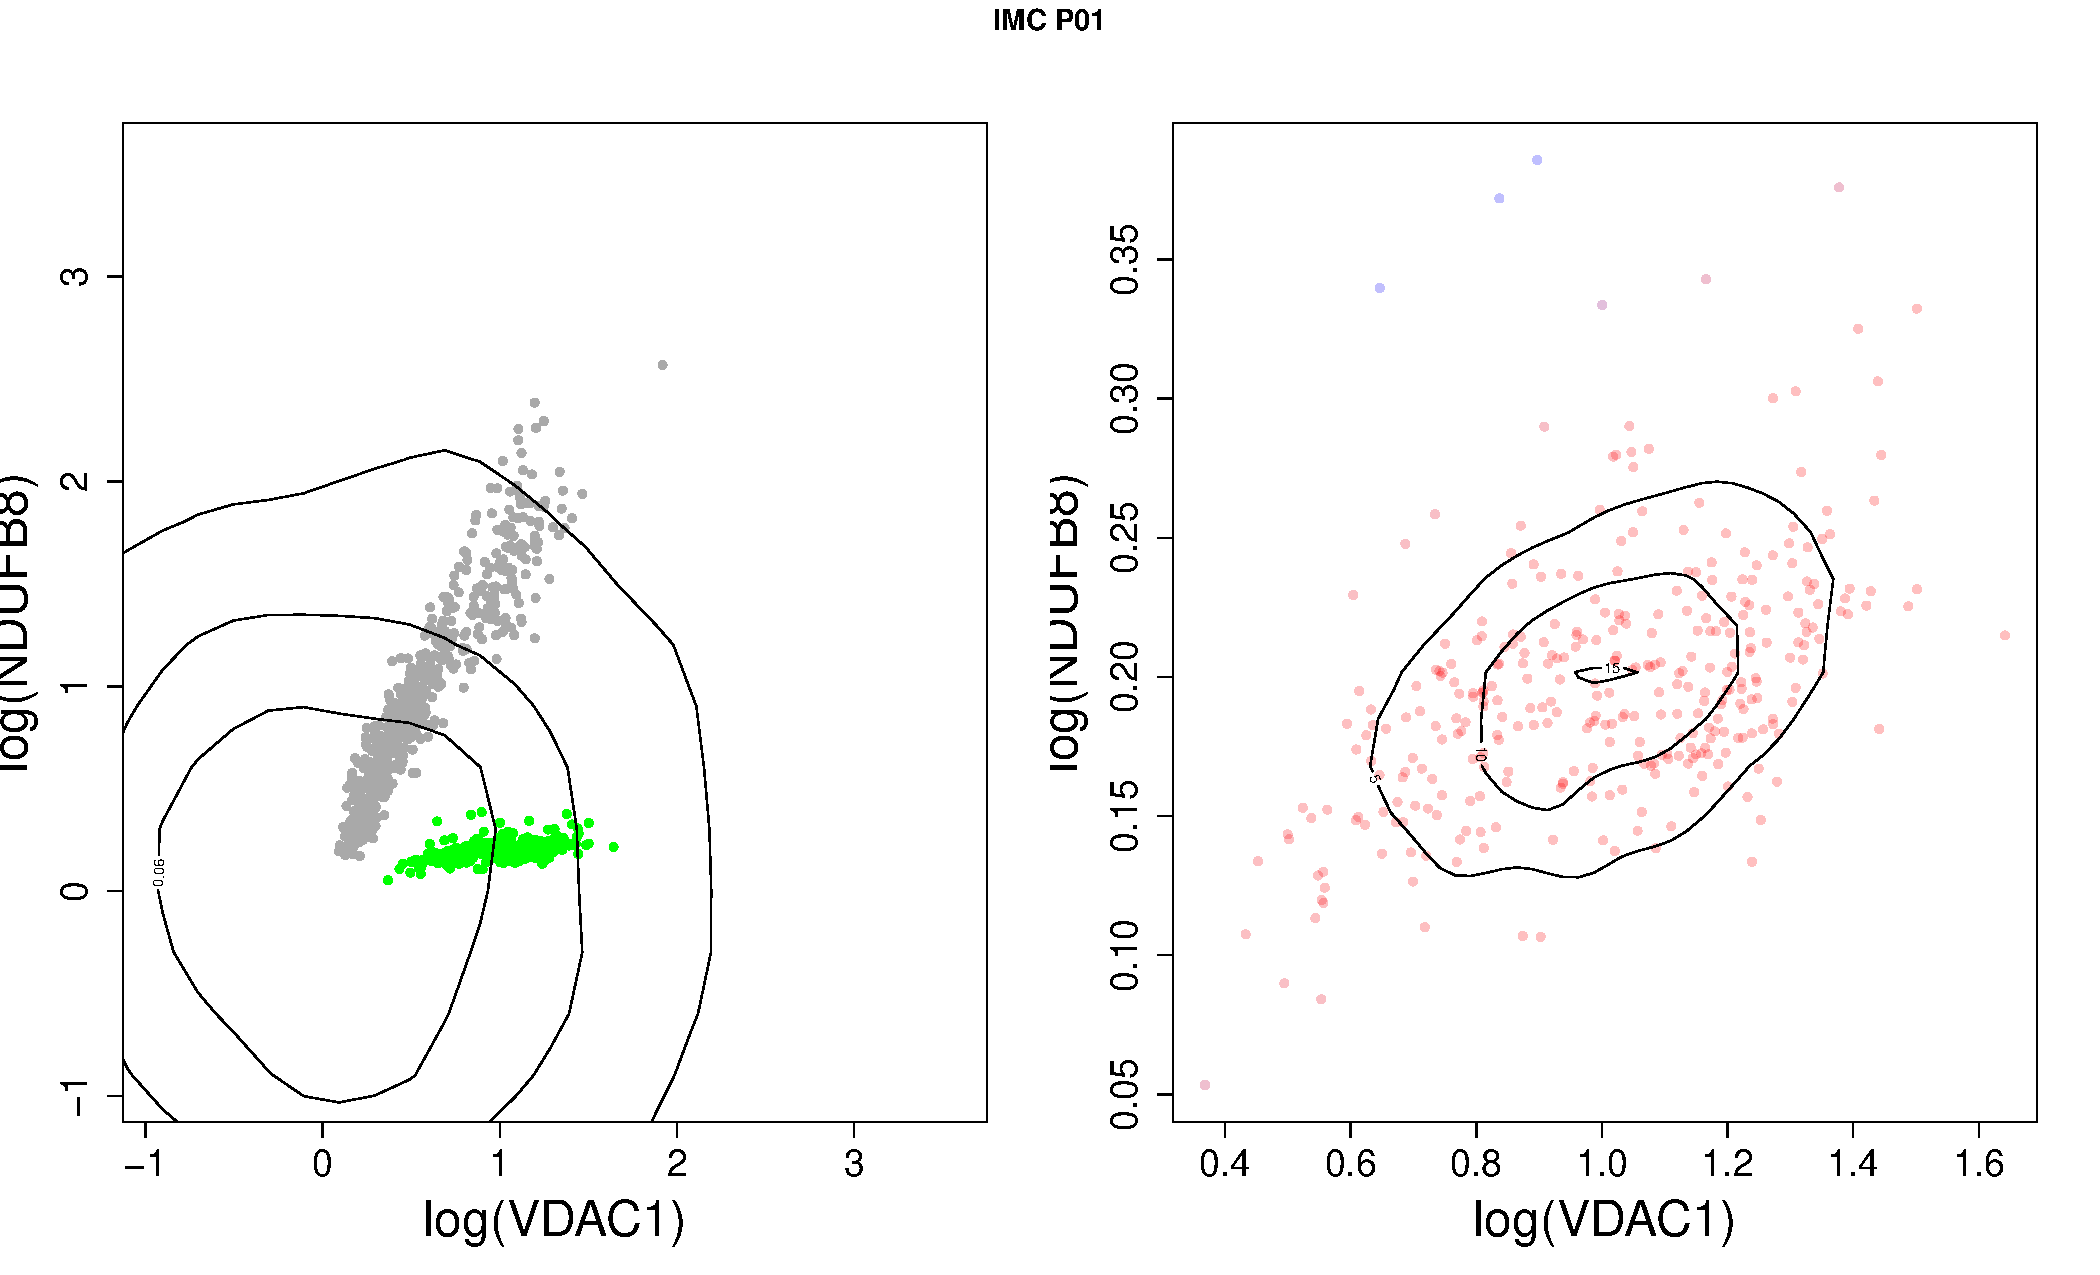
\includegraphics[width=0.8\textwidth]{IMC__P01__NDUFB8.pdf}
    \caption{10,000 draws from the prior and posterior densities about the distribution of NDUFB8 protein in healthy patients.}
    \label{fig:imc_control_ndufb8}
\end{figure}

\section*{Patient Data}
\subsection*{Prior Beliefs}
We choose priors for the patient data based on information from the posterior distributions for the control data. This is only for component one (`like control'). 
\begin{equation}
    \boldsymbol{\mu}_1 \sim \text{N}\left( \text{mean}(\tilde{\boldsymbol{\mu}}),  100*\text{var}(\tilde{\boldsymbol{\mu}})\right),
\end{equation}
where $\tilde{\boldsymbol{\mu}}$ denotes the set of draws from the posterior distribution of $\boldsymbol{\mu}_1$ from the control inference. The variance matrix is increased by a factor of 100 to allow for differences between the patient and control data. The variance parameter $T_1$, is again given a Wishart distribution, designed to have an expected value ten times greater than the control.
\begin{equation}
    T_1 \sim \text{Wishart}\left(10, \text{mean}(\tilde{T}) \right).
\end{equation}
For a Wishart distribution with parameters $V$, a positive definite matrix, and degrees of freedom $n$, the expectation is $nV$. \\

The parameters for the second component are given the following priors. 
\begin{center}
   \begin{tabular}{c  c}
    $\boldsymbol{\mu}_2 \sim \text{N}\left( 2*\text{mean}(\tilde{\boldsymbol{\mu}_1}), \begin{pmatrix}6&0\\0&6 \end{pmatrix}\right),$ & $T_2 \sim \text{Wishart}\left(3, \begin{pmatrix}2&0\\0&2\end{pmatrix} \right) $  \\
\end{tabular} 
\end{center}
As an example Figure \ref{fig:imc_p01_ndufb8_pri} shows the prior beliefs for Patient 01 (P01).

\begin{figure}[H]
    \centering
    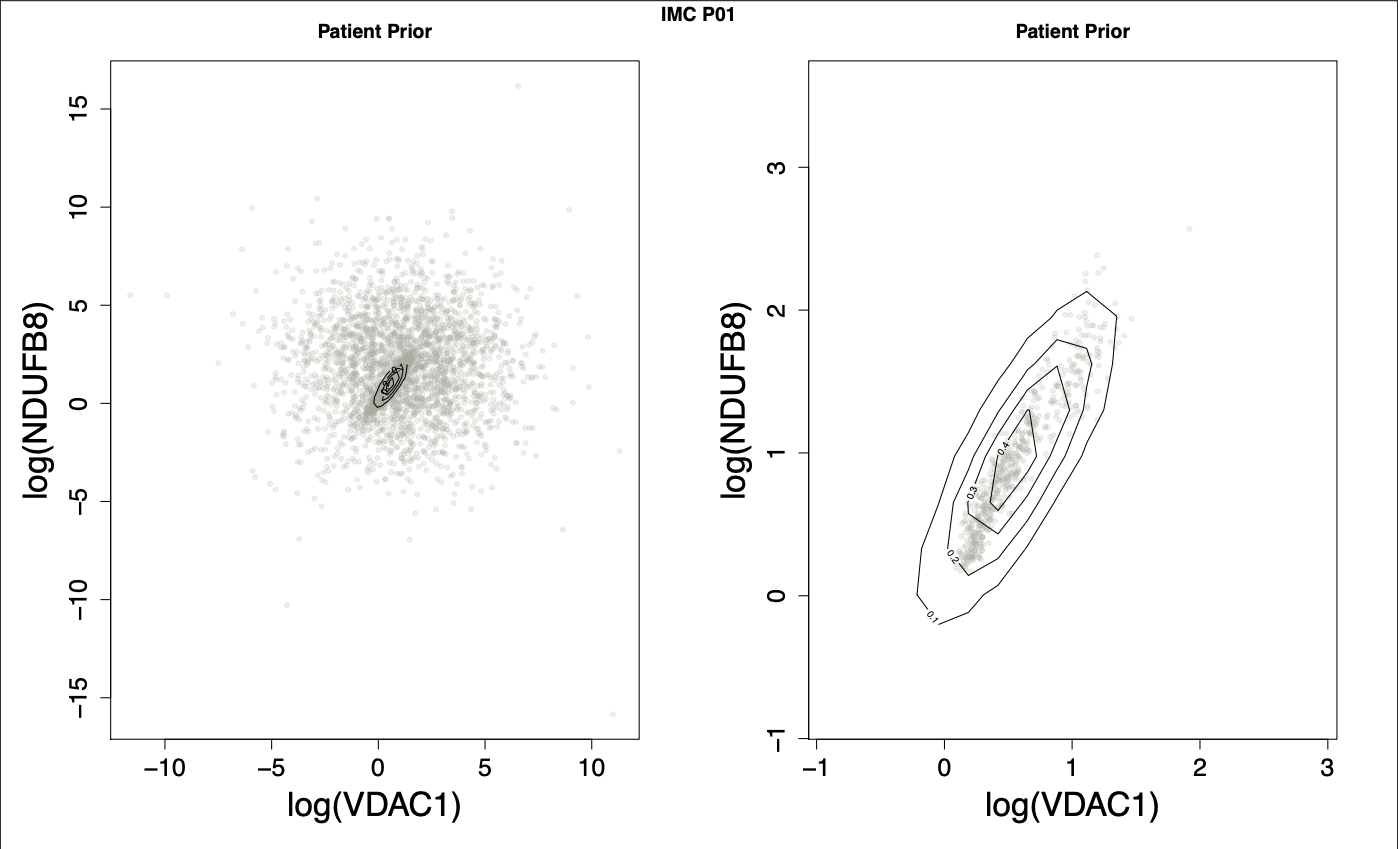
\includegraphics[width=0.8\textwidth]{IMC_P01_NDUFB8_prior.png}
    \caption{(Left) Prior beliefs for the expression of the NDUFB8 protein in a patient. (Right) Prior density and patient data for P01.}
    \label{fig:imc_p01_ndufb8_prior}
\end{figure}

\subsection*{Posterior Beliefs}

The example of 

\end{document}
